\graphicspath{{./figures/}}
\title{}
\date{}
\begin{document}
\begin{frame}
    \titlepage
\end{frame}


{
\setbeamercolor{background canvas}{bg=blue!40!black,fg=blue!10!white}
\setbeamercolor{normal text}{bg=blue!40!black,fg=blue!10!white}
\setbeamercolor{itemize/enumerate body}{fg=white}
\setbeamercolor{itemize/enumerate subbody}{fg=white}
\setbeamercolor{titlelike}{bg=blue!40!black,fg=blue!10!white}
\begin{frame}<1|handout:1>[noframenumbering]{Changelog}
    \begin{itemize}
    \item 3 May 2021: adjust phrasing about in-edges on `control flow graph' slide
    \item 3 May 2021: CFI prevents exercise: add explanation + E. none of these options
    \item 3 May 2021: Android shadow stacks: adjust font size of references
    \item 3 May 2021: clang CFI example: correct shown mask to have 5 entries
    \item 4 May 2021: CFI prevents exercise: add more explanations
    \end{itemize}
\end{frame}
}



\begin{frame}{last time}
    \begin{itemize}
    \item sandboxing integration with UI
        \begin{itemize}
        \item file selection outside sandbox as way to specify accessible files
        \item Qubes --- marking of `which sandbox' via borders in UI
        \end{itemize}
    \item sandboxing without OS support
        \begin{itemize}
        \item compiling C/C++ code for language VMs
        \item key insight: keep bounds in sandbox, not in array in sandbox
        \end{itemize}
    \item interfaces for sandboxing?
    \item application permissions
        \begin{itemize}
        \item avoiding wasting user attention
        \item communicating what permissions do (or not)
        \item evading permissions via missed interfaces
        \item evading permissions via cooperation with other apps
        \end{itemize}
    \end{itemize}
\end{frame}

\begin{frame}{a correction}
    \begin{itemize}
    \item explained Cloak+Dagger incorrectly
    \vspace{.5cm}
    \item one issue: system alert + accessiblity permission = complete control
        \begin{itemize}
        \item hide app + interact on user's behalf
        \end{itemize}
    \item another issue: use system alert permission to hide all part of ``allow'' button
    \end{itemize}
\end{frame}

\begin{frame}{note on CHALLENGE}
    \begin{itemize}
    \item assignment released
    \item schedule showed wrong due time briefly -- 9PM on 12 May (not midnight)
    \end{itemize}
\end{frame}


% FIXME: Intel bounds checking extension
    % FIXME: reorder shadow stack stuffs

\section{summary of mitigations / more ideas?}
\begin{frame}{mitigations so far}
    \begin{itemize}
    \item stopping attacker from writing working code
        \begin{itemize}
        \item write XOR execute
        \item removing ``gadgets''
        \item address space layout randomization
        \end{itemize}
    \item validating/protecting code pointers
        \begin{itemize}
        \item stack canaries
        \item full RELRO (protect linker stub pointers, pointers within VTable)
        \item missing: doing this for other code pointers?
        \item address space layout randomization
        \end{itemize}
    \item preventing out-of-bounds accesses
        \begin{itemize}
        \item guard pages
        \end{itemize}
    \end{itemize}
\end{frame} 

\begin{frame}{mitigation practicality concerns}
    \begin{itemize}
    \item backwards compatibility
        \begin{itemize}
        \item (high) works with unmodified libraries+programs
        \item sometimes works with unmodified libraries+program
            \begin{itemize}
            \item as long as they don't do something `weird'
            \end{itemize}
        \item requires recompile of module to be protected
        \item changes calling conventions: recompile module + things linked with it
        \item (low) requires changing source code
        \end{itemize}
    \item hardware support required
    \item extra space required
    \item extra time required
    \end{itemize}
\end{frame}

\begin{frame}{other mitigation ideas?}
    \begin{itemize}
    \item some big categories we haven't seen:
    \vspace{.5cm}
    \item protecting code pointers w/o vulnerability to information leaks
    \item validating/protecting non-return address code pointers
    \item preventing out-of-bounds accesses
    \end{itemize}
\end{frame}


\section{alternate mitigation: shadow stacks}
\usetikzlibrary{arrows.meta,shapes.multipart,patterns}

\begin{frame}{intuition: shadow stacks}
    \begin{itemize}
    \item problem with stack: easy to leak address/values because used for lots of data
    \vspace{.5cm}
    \item goal: keep sensitive data in \textbf{separate region}
        \begin{itemize}
        \item easier to kepe address secret?
        \end{itemize}
    \vspace{.5cm}
    \item can use this for (stronger?) alternative to stack canaries
    \end{itemize}
\end{frame}

\tikzset{
    stackBox/.style={very thick},
    onStack/.style={thick},
    frameOne/.style={fill=blue!15},
    frameTwo/.style={fill=red!15},
    markLine/.style={blue!50!black},
    markLineB/.style={red!90!black},
    hiLine/.style={red!90!black},
}
\begin{frame}{shadow stacks}
    \begin{tikzpicture}
    \tikzset{
        mainSt/.style={fill=blue!20},
        otherSt/.style={fill=yellow!20},
        every node/.style={font=\small,align=center},
    }
    \draw[stackBox,mainSt] (0, 0) rectangle (5, -6);
    \node[anchor=south] at (2.5, 0) { main stack @ \\ \texttt{0x7 0000 0000}};
    \begin{scope}[yshift=-.25cm]
    \draw[onStack] (0, 0) rectangle (5, -1.5) node[midway] {local variables for \texttt{foo}};
    \draw[onStack] (0, -1.5) rectangle (5, -2) node[midway] {arguments for \texttt{bar}};
    \draw[onStack] (0, -2) rectangle (5, -3.5) node[midway] {local variables for \texttt{bar}};
    \draw[onStack] (0, -3.5) rectangle (5, -4.0) node[midway] {arguments for \texttt{baz}};
    \draw[red,very thick,Latex-] (5.25, -4.0) -- ++(.5, 0) node[right] {stack pointer};
    \end{scope}
    \node[anchor=south] at (9, 0) { `shadow' stack @ \\ \texttt{0x8 0000 0000}};
    \draw[stackBox,otherSt] (6.5, 0) rectangle (11.5, -3);
    \begin{scope}[yshift=-.25cm,xshift=6.5cm]
    \draw[onStack] (0, 0) rectangle (5, -0.5) node[midway] {return address for \texttt{foo}};
    \draw[onStack] (0, -0.5) rectangle (5, -1) node[midway] {return address for \texttt{bar}};
    \draw[onStack] (0, -1) rectangle (5, -1.5) node[midway] {return address for \texttt{baz}};
    \draw[red,very thick,Latex-] (5.25, -1.5) -- ++(.5, 0) node[right] {shadow \\stack pointer};
    \end{scope}
    \end{tikzpicture} 
\end{frame}

\begin{frame}{implementing shadow stacks}
    \begin{itemize}
    \item bigger changes to compiler than canaries
    \item more overhead to call/return from function
    \item most commonly: store return address twice
    \end{itemize}
\end{frame}

\begin{frame}[fragile,label=shadowStackx8664v1]{shadow stacks on x86-64 (1)}
\begin{itemize}
\item idea 1: dedicate \%r15 as shadow stack pointer, \\
      copy RA to shadow stack pointer in function prologue
\end{itemize}
\begin{lstlisting}[language=myasm]
function:
    movq (%rsp), %rax    // RAX <- return address
    addq $-8, %r15       // R15 <- R15 - 8
    movq %rax, (%r15)    // M[R15] <- RAX
    ...
    movq (%rsp), %rdx     // RDX <- return address
    cmpq %rdx, (%r15)    
    jne CRASH_THE_PROGRAM // if RDX != M[R15] goto CRASH_THE_PROGRAM
    add $8, %r15          // R15 <- R15 - 8
    ret
\end{lstlisting}
\end{frame}

\begin{frame}[fragile,label=shadowStackx8664v2]{shadow stacks on x86-64 (2)}
\begin{itemize}
\item idea 2: dedicate \%r15 as shadow stack pointer, \\
      avoid normal call/return instruction
\end{itemize}
\begin{lstlisting}[language=myasm]
    addq $-8, %r15
    leaq after_call(%rip), %rax
    movq %rax, (%r15)
    jmp function
after_call:

function:
    ...
    addq $8, %r15        // R15 <- R15 + 8
    jmp *-8(%r15)        // jmp M[R15-8]
\end{lstlisting}
\end{frame}

\begin{frame}[fragile,label=actShadowStack]{Android/AArch64 shadow stacks (1)}
   \begin{itemize}
    \item \tiny via \url{https://clang.llvm.org/docs/ShadowCallStack.html} (see also {\url{https://security.googleblog.com/2019/10/protecting-against-code-reuse-in-linux_30.html}})
    \item dedicate register \texttt{x18} to shadow stack pointer
        \begin{itemize}
        \item x30 = return address (after ARM's call instruction (bl))
        \end{itemize}
    \item ARM call instruction saves return address in register\ldots
    \end{itemize}
\begin{tikzpicture}
\node[draw,label={with shadow stack}] (code1) {
\begin{lstlisting}[language={},style=script]
str     x30, [x18], #8      
stp     x29, x30, [sp, #-16]!
mov     x29, sp
bl      bar
add     w0, w0, #1
ldp     x29, x30, [sp], #16
ldr     x30, [x18, #-8]!
ret
\end{lstlisting}
};
\node[anchor=north east,draw,label={without}] (code2) at (code1.north west) {
\begin{lstlisting}[language={},style=script]
stp     x29, x30, [sp, #-16]!
mov     x29, sp
bl      bar
add     w0, w0, #1
ldp     x29, x30, [sp], #16
ret
\end{lstlisting}
};
\end{tikzpicture}
\end{frame}



\subsection{Intel's hardware support?}
\begin{frame}{Intel CET shadow stacks}
    \begin{itemize}
    \item future Intel processor extension adds shadow stacks
        \begin{itemize}
        \item ``Control-flow Enforcement Technology''
        \end{itemize}
    \vspace{.5cm}
    \item new shadow stack pointer
    \item CALL/RET: push/pop from BOTH stacks
    \item shadow stack pages are marked as read-only in page table
        \begin{itemize}
        \item cannot be written through normal instructions
        \item extra bit identifying as shadow stack (not ``normal'' read-only page)
        \end{itemize}
    \end{itemize}
\end{frame}


\subsection{can we prevent writes now?}
\begin{frame}{preventing shadow stack writes?}
\begin{itemize}
\item ARM64 scheme: prevent writes if
    \begin{itemize}
    \item shadow stack pointer is never leaked (dedicated register)
    \item shadow stack random location can't be guessed (or queried otherwise)
    \end{itemize}
\item Intel CET: prevent writes unless
    \begin{itemize}
    \item OS (priviliged/kernel mode) instructions to setup shadow stack used
    \end{itemize}
\vspace{.5cm}
\item can we prevent writes without relying on avoiding info leaks\ldots \\
      and without special hardware support?
      \begin{itemize}
      \item well, yes, but \ldots
      \end{itemize}
\end{itemize}
\end{frame}

\begin{frame}{some early stack canary benchmarks}
{\small from Chiueh and Hsu, ``RAD: A Compile-Time Solution to Buffer Overflow Attacks'' (2001)}
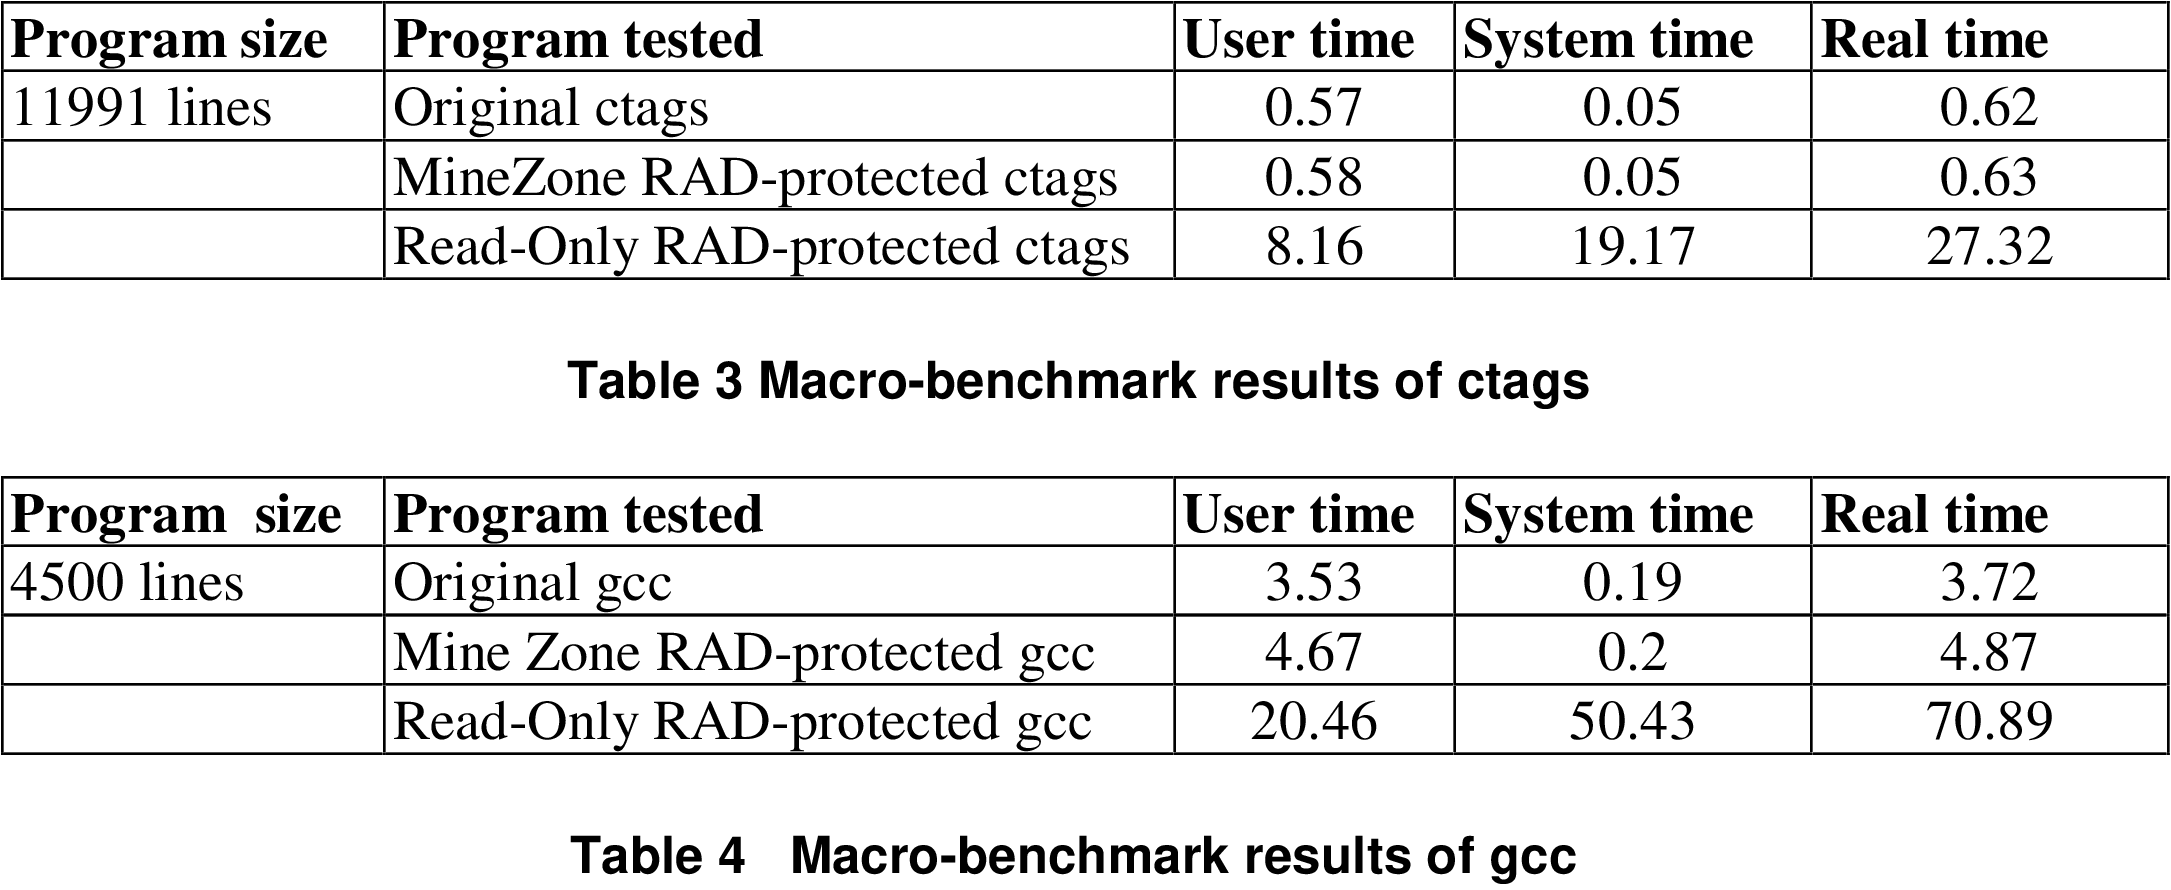
\includegraphics[height=0.8\textheight]{../mitigate/rad-results}
\end{frame}



\subsection{exceptions, setjmp, etc.}
\usetikzlibrary{arrows.meta,patterns}

\begin{frame}{automatic shadow stacks?}
    \begin{itemize}
    \item if we change how CALL/RET works\ldots
    \item \ldots maybe we can add shadow stack support to existing programs?
    \begin{itemize}
        \item either with hardware support, or
        \item in software with emulation techniques?
        \end{itemize}
    \vspace{.5cm}
    \item well, there's a problem\ldots
    \end{itemize}
\end{frame}


\begin{frame}[fragile,label=noAutomaticStack1]{the problem in C++}
\begin{lstlisting}[language=C++,style=smaller]
void Foo() {
    try {
        ... Bar() ...
    } except (std::runtime_error &error) {
        ...
    }
}

void Bar() {
    ... Quux() ...
}
void Quux() {
    ...
    throw std::runtime_error("...");
    ...
}
\end{lstlisting}    
\end{frame}

\begin{frame}[fragile,label=noAutomaticStack2]{the problem in C}
\begin{lstlisting}[language=C++,style=smaller]
jmp_buf env;
const char *error;
void Foo() {
    if (0 == setjmp(env)) {
        Bar();
    } else {
        ...
    }
}

void Bar() {
    ... Quux() ...
}
void Quux() {
    ...
    error = "...";
    longjmp(env, 1);
    ...
}
\end{lstlisting}    
\end{frame}

\begin{frame}{dealing with non-local returns}
\begin{itemize}
\item exceptions and setjmp/longjmp deliberately skip return calls
\item one solution: ``direct'' shadow stack
\item fixed (possibly secret) offset from normal stack
\item shadow stack only stores return addreses
    \begin{itemize}
    \item space in between return addresses left as nulls
    \end{itemize}
\end{itemize}
\begin{tikzpicture}[overlay,remember picture]
\coordinate (top) at ([xshift=-5cm,yshift=-2.5cm]current page.north east);
\draw[very thick] (top) rectangle ++(4cm, -7cm);
\draw[thick,pattern=north west lines] (top) ++(0cm, -1cm) rectangle ++(4cm, -2cm) node[yshift=-0.5cm,midway,fill=white] {shadow stack};
\draw[thick,pattern=north west lines] (top) ++(0cm, -4cm) rectangle ++(4cm, -2cm) node[yshift=-0.5cm,midway,fill=white] {normal stack};
\draw[thick,fill=blue!20] (top) ++(0cm, -1.4cm) rectangle  ++(4cm, -0.1cm) coordinate (after shadow ra);
\draw[thick,fill=blue!20] (top) ++(0cm, -4.4cm) rectangle  ++(4cm, -0.1cm) coordinate (after ra);
\draw[thick,fill=blue!20] (top) ++(0cm, -1.1cm) rectangle  ++(4cm, -0.1cm);
\draw[thick,fill=blue!20] (top) ++(0cm, -4.1cm) rectangle  ++(4cm, -0.1cm);
\draw[thick,fill=orange!20] (top) ++(0cm, -4.2cm) rectangle  ++(4cm, -0.2cm);
\draw[thick,fill=orange!20] (top) ++(0cm, -4cm) rectangle  ++(4cm, -0.1cm);
\node[anchor=north,font=\small,fill=white] at ([xshift=-2cm]after shadow ra) {shadow RA};
\node[anchor=north,font=\small,fill=white] at ([xshift=-2cm]after ra) {return addr};
\path[draw,very thick,-Latex] (after ra) -- ++(.25cm,0cm) |- (after shadow ra);
\end{tikzpicture}
\end{frame}


\subsection{exercise: shadow stacks stop}
\begin{frame}{what do shadow stacks stop?}
    \begin{itemize}
    \item combined with a information leak that can dump arbitrary bytes of memory, \\
       which of these exploits would shadow stacks stop\ldots
    \begin{itemize}
    \item A. using format string exploit to point stack return address to the `system' function
    \item B. using format string exploit to point VTable to the `system' function
    \item C. using an unchecked string copy that goes over the end of a stack buffer into the return address and pointing the return address to the `system' function
    \item D. using a buffer overflow that overwrites a saved stack pointer value to cause return to use a different address
    \item E. using pointer subterfuge to overwrite the GOT entry for `printf' to point to the `system' function
    \end{itemize}
    \end{itemize}
\end{frame}


\section{simple control flow integrity}

\subsection{idea: checking returns?}

\begin{frame}{a simple way to check returns?}
\begin{itemize}
\item observation: places we return to usually after call instructions
    \begin{itemize}
    \item exception: `tail calls' --- we'll ignore this for now
    \end{itemize}
\vspace{.5cm}
\item we could check for one\ldots
\item replace return with:
\end{itemize}
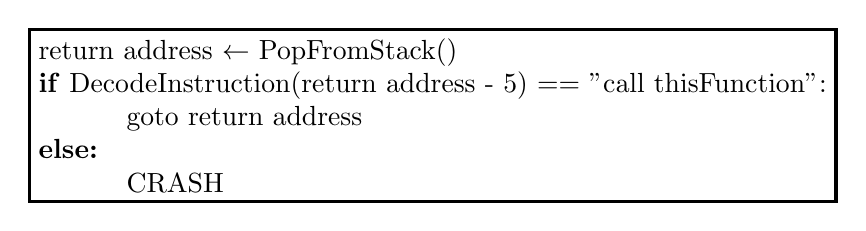
\begin{tikzpicture}
\node[align=left,draw,very thick] {
return address $\leftarrow$ PopFromStack() \\
\textbf{if} DecodeInstruction(return address - 5) == "call thisFunction": \\
\hspace{1cm} goto return address \\
\textbf{else:} \\
\hspace{1cm} CRASH
};
\end{tikzpicture}
\end{frame}

\begin{frame}[fragile,label=simCheckRetLabel]{a simple way to check returns?}
\begin{itemize}
\item more practical: \texttt{label \$ID} instruction with encoding:
    \begin{itemize}
    \item \texttt{TWO-BYTE-OPCODE} \texttt{FOUR-BYTE-CONSTANT}
    \item (real version: can reuse some sufficiently nop-like instruction)
    \end{itemize}
\end{itemize}
\begin{tikzpicture}
\node[font=\tt,align=left,draw,very thick] (the call) {
\begin{lstlisting}[language=myasm,style=smaller]
...
    call foo
    label $0xf19279bb // random ID for function foo
...
\end{lstlisting}
};
\node[align=left,anchor=north west,draw,very thick] at ([yshift=-1cm]the call.south west) {
\begin{lstlisting}[language=myasm,style=smaller]
foo: 
...
    pop %rdx          // RDX <- return address
    cmp $0xf19279bb, 2(%rdx) 
    jne CRASH
    jmp *%rdx
\end{lstlisting}
};
\end{tikzpicture}
\end{frame}


    % FIXME: verify that it's after a call instruction
        
        % FIXME: same idea, but mark the return sites explicitly
    % FIXME: verify that it's after a call isntruction for the right function
        % FIXME: same idea, but mark the return sites explicitly

\subsubsection{versus canaries?}
\begin{frame}{looks like canaries? (1)}
    \begin{itemize}
    \item what attacks does this stop that canaries don't?
    \vspace{.5cm}
    \item<2-> ID does not need to be secret!
        \begin{itemize}
        \item<2-> assuming non-executable writeable memory, no!
        \item<2-> attacker can't write new places for return to go
        \end{itemize}
    \item<3-> avoids ``stack pivoting'' attacks
        \begin{itemize}
        \item attacker can't make stack pointer point to wrong part of stack\ldots
        \item and expect it to return differently
        \end{itemize}
    \end{itemize}
\end{frame}

\begin{frame}[fragile,label=cfiLikeCanariesP2]{looks like canaries? (2)}
    \begin{itemize}
    \item what attacks does this NOT stop that canaries don't?
    \item example: SortList can be called from \texttt{Innocent}, \\ then return from \texttt{Dangerous}
        \begin{itemize}
        \item assumption: attacker can overwrite return address at right time (running on another core? problem with sortFunc1?)
        \end{itemize}
    \end{itemize}
\begin{tikzpicture}
\node[draw,very thick,align=left] (a) {
\begin{lstlisting}[language=C++,style=smaller]
void Innocent() {
  ...
  SortList(someList1,
           sortFunc1);
  Use(someList1);
  ...
}
\end{lstlisting}
};
\node[draw,very thick,align=left,anchor=north west] at ([xshift=1cm]a.north east) (b) {
\begin{lstlisting}[language=C++,style=smaller]
void Dangerous() {
  ...
  SortList(someList2,
           sortFunc2);
  UseDangerously(someList2);
  ...
}
\end{lstlisting}
};
\end{tikzpicture}
\end{frame}


\subsection{checking VTable calls?}
    % FIXME: applying idea to calls to VTable-based function call
\begin{frame}[fragile,label=checkVTable1]{checking a VTable call}
\begin{tikzpicture}
\node[draw,very thick,align=left] (base c code) {
\begin{lstlisting}[language=C++,style=smaller]
class A { public:
  virtual void bar() { ... }
};
class B : public A { public:
  void bar() { ... }
};
void example(A *obj) {
  obj->bar();
}
\end{lstlisting}
};
\node[draw,very thick,anchor=north west,align=left] (base asm code) at ([yshift=-.25cm] base c code.south west) {
\begin{lstlisting}[language=myasm,style=smaller]
example:
  // rax <- vtable address
  movq (%rdi), %rax
  // rdx <- first vtable entry
  movq (%rax), %rax
  // call using vtable entry
  call *%rax
  ...
\end{lstlisting}
};
\begin{visibleenv}<2>
\node[draw=red,very thick,anchor=north west,align=left,font=\fontsize{12}{13}\selectfont] (warning) at ([xshift= .5cm]base asm code.north east) {
example uses VTable to call method \\
target for memory corruption attacks \\
just like return addresses \\
so, apply same strategy
};
\end{visibleenv}
\begin{visibleenv}<3->
\node[draw=red,very thick,anchor=north west,align=left] (new asm code) at ([xshift= .5cm]base asm code.north east) {
\begin{lstlisting}[language=myasm,style=smaller]
example:
  movq (%rdi), %rax
  movq (%rax), %rax
  cmpq $0xe0c5df0b, 2(%rax)
  jne CRASH
  call *%rax
  ...
\end{lstlisting}
};
\node[draw=red,very thick,anchor=south west,align=left] (new method code) at ([yshift=.5cm]new asm code.north west) {
\begin{lstlisting}[language=myasm,style=smaller]
A::bar():
  label $0xe0c5df0b
  ...
B::bar():
  label $0xe0c5df0b
  ...
\end{lstlisting}
};
\end{visibleenv}
\end{tikzpicture}
\end{frame}


\subsection{checking VTable call returns?}
    % FIXME
\begin{frame}[fragile,label=checkVTableRet1]{checking a VTable return}
\begin{tikzpicture}
\node[very thick,anchor=north west,align=left] (base asm code) {
\begin{lstlisting}[
    language=myasm,style=smaller,
    moredelim={**[is][\btHL<1->]{~1~}{~end~}},
]
example:
  movq (%rdi), %rax
  movq (%rax), %rax
  cmpq $0xe0c5df0b, 2(%rax)
  jne CRASH
  call *%rax
  ~1~label $0x64a0cfe3~end~
  ret
\end{lstlisting}
};
\node[very thick,anchor=north east,align=left] (base method code) at ([xshift=.5cm]base asm code.north west) {
\begin{lstlisting}[language=myasm,style=smaller,
    moredelim={**[is][\btHL<1->]{~1~}{~end~}},
]
A::bar():
  label $0xe0c5df0b
  ...
  ~1~pop %rdx~end~ // RDX <- return address
  ~1~cmp $0x64a0cfe3, 2(%rdx)~end~
  jne CRASH
  jmp *%rdx
B::bar():
  label $0xe0c5df0b
  ...
  ~1~pop %rdx~end~ // RDX <- return address
  ~1~cmp $0x64a0cfe3, 2(%rdx)~end~
  jne CRASH
  jmp *%rdx
\end{lstlisting}
};
\node[draw=red,very thick,anchor=north west,align=left] at ([yshift=-.5cm]base method code.south west) {
if we want to use this label-checking on the return \\
need to choose the same label for A::bar and B::bar return, too
};
\end{tikzpicture}
\end{frame}


\subsection{checking indirect function calls}
    % FIXME: trivial idea: was there a pointer?
        % well, that's not very nice\ldots
\begin{frame}[fragile,label=checkIndirectSortIntro]{calls through function pointers}
\begin{lstlisting}[language=C++,style=small]
typedef int (*CompareFnType)(const char*, const char*)
void SortFunction(const char **items, CompareFnType compare) {
    ...
    (*compare)(a, b);
    ...
}
\end{lstlisting}
\begin{itemize}
\item here: call through explicitly passed function pointer
\item want to do the same thing we did for VTable calls
    \begin{itemize}
    \item all the compare functions have the same label
    \item all the returns form compare functions have the same label
    \end{itemize}
\vspace{.5cm}
\item yes, \myemph<2->{if we can somehow label all the compare functions}
\end{itemize}
\end{frame}



\section{CFI overhead}
\begin{frame}{CFI overhead}
\begin{itemize}
\item Abadi et al's 2004 paper:
    \begin{itemize}
    \item used label-based approach
    \item 0-45\% time overhead on SPECcpu2000 benchmarks
    \item best: compression program
    \item worst: chess engine
    \end{itemize}
\item Tice et al's 2014 paper (clang-style impl, sometimes in GCC, sometimes in Clang)
    \begin{itemize}
    \item could seperately enable different parts
    \item in tests on SPECcpu 2006 benchmarks:
    \item 0--10\% slowdown for VTable dereference checks 
        \begin{itemize}
        \item but 20\% without tuning
        \end{itemize}
    \item 0-6\% for other indirect call checking
    \end{itemize}
\end{itemize}
\end{frame}


\section{what does CFI actually prevent}
\againframe<2>{cfiLikeCanariesP2}

\section{more general control flow integrity}

\subsection{concept: control flow graph}
\usetikzlibrary{calc}
\begin{frame}{concept: labels and control flow graph}
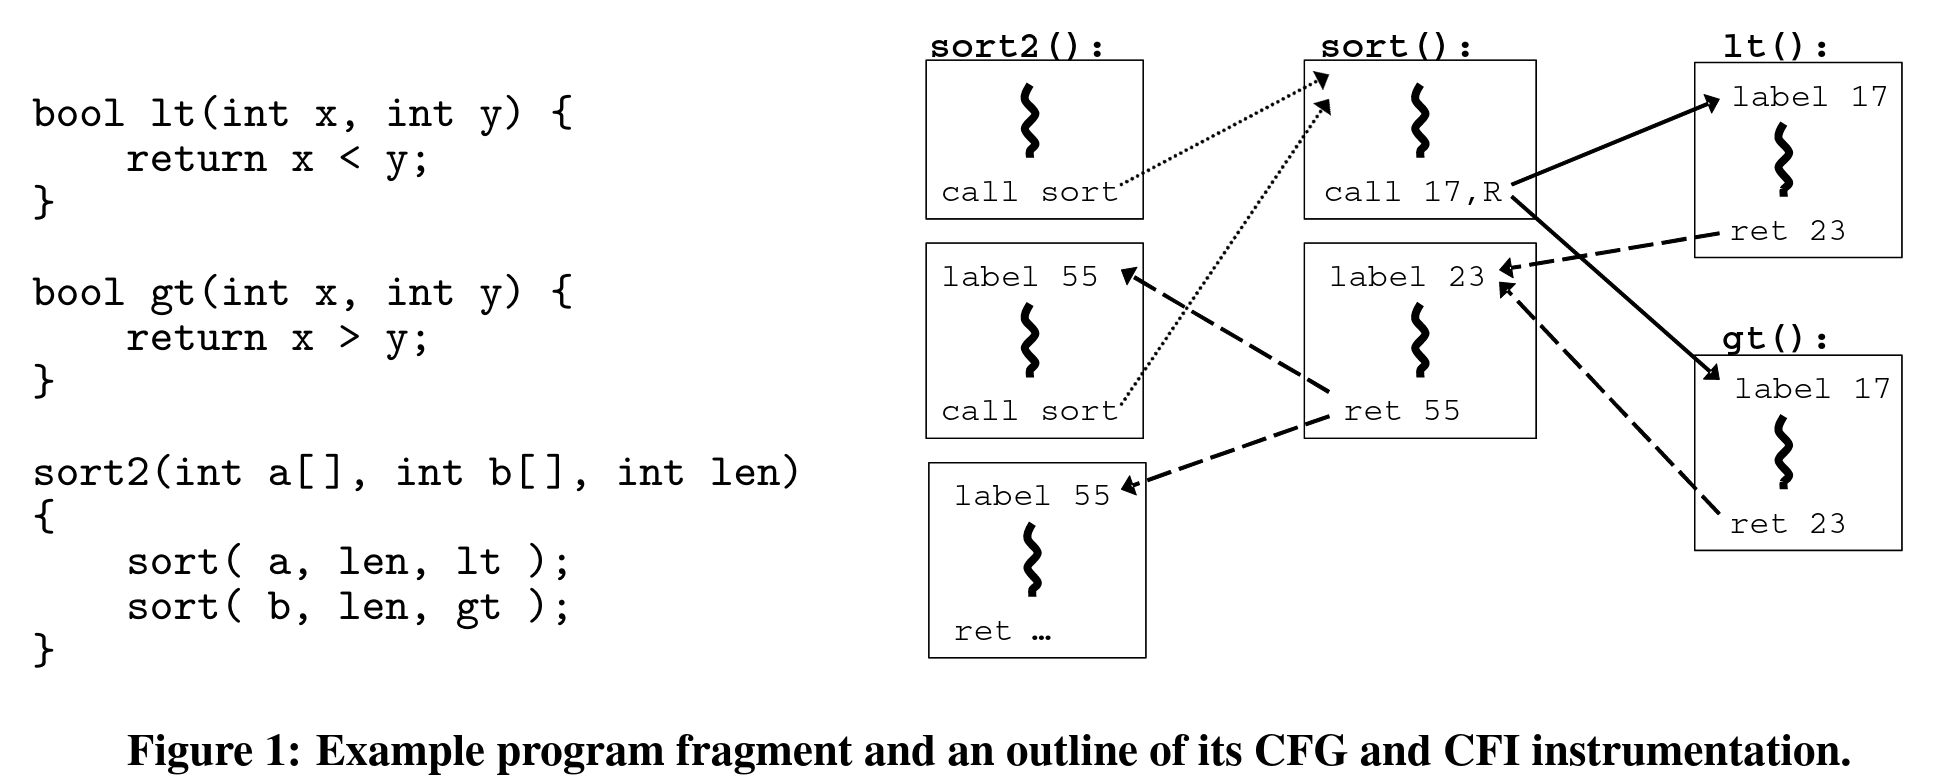
\includegraphics[width=0.7\textwidth]{../cfi/abadi-fig1}
\begin{itemize}
\item control flow graph
    \begin{itemize}
    \item nodes = blocks of code
    \item edges = \textit{potential jump/call}
    \end{itemize}
\item assigning labels: every in-edge needs to check same label at source
\end{itemize}
\imagecredit{figure from Abadi et al, ``Control-Flow Integrity: Principles, Implementations and Applications'' (CCS 2005)}
\end{frame}

 % FIXME: needs explanation of how labels assigned

\subsection{and function pointers}

\usetikzlibrary{arrows.meta}

\begin{frame}[fragile,label=tracking]{library-crossing CFGs}
\begin{tikzpicture}
\node[draw,very thick,label={north:main.c}] (mainc) {
\begin{lstlisting}[language=C++,style=script]
#include <png.h>
void ReadImageFromNetwork(
    png_structp libpng_handle,
    unsigned char *bytes,
    size_t size
) { ...  }

int main() {
    /* init libpng */
    png_structp libpng_handle = ...;
    /* tell libpng how to read image data */
    png_set_read_fn(
        libpng_handle, ...,
        ReadImageFromNetwork
    )
    ...
    /* extract "header" 
       information from image */
    png_get_IHDR(libpng_handle, ...)
    ...
}
\end{lstlisting}
};
\coordinate (base) at ([xshift=.5cm]mainc.north east);
\begin{scope}[shift=(base)]
    \tikzset{
        every node/.style={draw,align=left,font=\fontsize{10}{11}\tt\selectfont},
    }
    \node[draw,align=left,text width=1.25cm,anchor=north west] (main1) at (0,0) {
        main: \\
        ... \\
    };
    \node[draw,align=left] (set read) at (4, -1.5) {
        png\_set\_read\_fn: \\
        ... \\
        ...
    };

    \node[draw,align=left,text width=1.25cm,anchor=north west] (main2) at (0,-3) {
        ... \\
    };
    \draw[-Latex,very thick] (main1) -- (set read);
    \draw[-Latex,very thick] (set read) -- (main2);
    \node[draw,align=left] (ihdr) at (4, -4) {
        png\_get\_IHDR: \\
        ... \\
    };
    \node[draw,align=left] (readFromNet) at (5, -6) {
        ReadImage\\FromNetwork: \\
        ... 
    };
    \draw[-Latex,very thick] (main2) -- (ihdr);
    \draw[-Latex,very thick] (ihdr) -- (readFromNet);

    \begin{pgfonlayer}{bg}
    \draw[ultra thick,black!50,dotted,fill=blue!10] (-0.25,0.25) -- (1.9,0.25) -- (1.9,-5.2) -- (6.75,-5.2) --
        (6.75, -7) -- (-0.25,-7) -- cycle;
    \draw[ultra thick,black!50,dotted,fill=yellow!10] (2,-.5) -- (6.5,-.5) -- (6.5, -5) -- (2, -5) -- cycle;
    \end{pgfonlayer}
\end{scope}
\end{tikzpicture}
\end{frame}

\begin{frame}[fragile,label=imprecise]{CFGs will be imprecise}
\begin{lstlisting}[language=C++,style=smaller]
FunctionPtr p = functionA;
Example() {
  while (true) {
    ...
    if (SomethingComplicated()) {
      (*p)();
    } else if (SomethngElseComplicated()) {
      foo();
    }
    ...
  }
}
foo() {
  ...
  if (AnotherComplexThing()) {
    p = functionB;
  }
}
\end{lstlisting}
\begin{itemize}
\item can Example() call functionB()? probably not practical to tell
    \begin{itemize}
    \item need to make conservative `yes' guess
    \end{itemize}
\end{itemize}
\end{frame}


\subsection{finding function pointer values?}
\begin{frame}[fragile,label=fptrValues]{finding possible function pointer values?}
\begin{itemize}
\item given call using function pointers \\
how do we find the \textbf{legitimate} possible values?
\item one idea:
\end{itemize}
\begin{lstlisting}[language={},style=smaller,
    moredelim={**[is][\btHL<2-|handout:0>]{~2~}{~end~}},
]
for each fptr constant X: PossibleValues[X] = {X}
for each fptr ~2~variable X~end~:
    PossibleValues[X] = empty set
until PossibleValues stops changing:
    for each fptr assignment LHS=RHS:
        for ~2~each fptr variable/constant Y~end~
                ~2~that RHS could evaluate to~end~:
            PossibleValues[LHS] = Union(
                PossibleValues[LHS],
                PossibleValues[Y]
            )
\end{lstlisting}
\end{frame}




% FIXME:
\subsection{imprecision: unions, etc.}
\usetikzlibrary{arrows.meta}

\begin{frame}{labels aren't enough?}
\begin{tikzpicture}
\begin{scope}
\tikzset{
    every node/.style={align=left,draw,very thick,font=\tt\fontsize{11}{12}\selectfont},
}
\node (foo) at (0, 0){
    foo: \\
    ... \\
    check for label ??? \\
    call *p 
};

\node (bar) at (1, -5) {
    bar: \\
    ... \\
    check for label ??? \\
    call *p
};

\node (A) at (6, -2) { A: \\ label ??? };
\node (B) at (6, -3) { B: \\ label ??? };
\node (C) at (6, -4) { C: \\ label ??? };

\begin{scope}[-Latex,thick]
\draw (foo.south east) -- (A.west);
\draw (foo.south east) -- (C.west);
\draw (bar.south east) -- (B.west);
\draw (bar.south east) -- (C.west);
\end{scope}
\end{scope}
\begin{visibleenv}<2->
\node[align=left,draw=red,ultra thick,anchor=north west] at (8, 0) {
two possible fixes: \\
~ \\
make checks scan \\
for multiple labels \\
(more overhead) \\
~ \\
allow foo to call B \\
and bar to call A \\
(easier to attack)
};
\end{visibleenv}
\end{tikzpicture}
\end{frame}


\section{Clang's CFI implementation}
\begin{frame}{clang's CFI implementation}
\begin{itemize}
\item \url{https://clang.llvm.org/docs/ControlFlowIntegrity.html}
    \begin{itemize}
    \item \scriptsize also \url{https://www.usenix.org/conference/usenixsecurity14/technical-sessions/presentation/tice}
    \end{itemize}
\item only checks calls via VTables or function pointers
\item stable implementation requires libraries compiled with support
\item label information is placed in separate data structure
    \begin{itemize}
    \item \myemph<2>{looked up using function} or VTable addresses
    \end{itemize}
\item trick: keep functions in one region of memory
\end{itemize}
\end{frame}

\begin{frame}[fragile,label=indirectDiag]{clang idea for CFI indirect calls}
\begin{tikzpicture}
\node[draw, very thick, align=left] (dispatcher) {
\begin{lstlisting}[language=myasm,style=smaller]
start_funcs_with_two_string_args:
.align 8
compare_alpha:
  jmp real_compare_alpha
.align 8
run_command_with_arg:
  jmp real_run_command_with_arg
.align 8
print_two_strings:
  jmp real_print_two_strings
.align 8
move_file:
  jmp real_move_file
.align 8
compare_reverse_alpha:
  jmp real_compare_reverse_alpha
end_funcs_with_two_sting_args:
\end{lstlisting}
};
\begin{visibleenv}<1>
\node[align=left,draw=red,very thick,anchor=north west] at ([xshift=1cm]dispatcher.north east) {
functions of same type \\
placed together \\
~ \\
every func's address \\
is multiple of 8
};
\end{visibleenv}
\begin{visibleenv}<2>
\node[align=left,draw=red,very thick,anchor=north west] at ([xshift=0.5cm]dispatcher.north east) {
check pseudocode: \\
round fptr to multiple of 8 \\
\textbf{if} fptr < start or fptr > end: \\
\hspace{1cm} CRASH \\
allowed $\leftarrow$ [1,0,0,0,1] \\
\hspace{0.5cm} \textit{`mask' for compare funcs} \\
offset $\leftarrow$ fptr - start \\
\textbf{if} bit (offset/8) of allowed \\
\hspace{2.5cm}is not set: \\
\hspace{1cm} CRASH
};
\end{visibleenv}
\end{tikzpicture}
\end{frame}

\begin{frame}{clang idea for VTables}
\begin{itemize}
\item check VTable element address instead of function address
\item otherwise
    \begin{itemize}
    \item place all VTables for related classes together
    \item check start/end address for VTables
    \item bit mask indicating which VTable entries are okay for call
    \end{itemize}
\end{itemize}
\end{frame}


\section{Clang's CFI prevents?}
\begin{frame}[fragile,label=cfiPrevents]{CFI prevents?}
\begin{lstlisting}[language=C++,style=script]
class Foo { public: virtual void f() { } };
class Bar : public Foo { public: virtual void f() { g(1); } };
class Quux : public Foo { public: virtual void f() { } };
void g(int x) { if (x == 0) { danger(); } }
int h(int x) { return 0; }
int (*ptr)(int) = &h;
\end{lstlisting}
\begin{itemize}
\item with clang's CFI, which likely can end up calling \texttt{danger()}
      if an attacker can first write to arbitrary memory locations?
    \begin{itemize}
    \item A. \lstinline|(*ptr)(1);| 
    \item B. \lstinline|(*ptr)(0);| \only<2->{\myemph{if compiler thinks ptr set to g ever, yes; otherwise, no}}
    \item C. \lstinline|Foo *q = attacker_controlled(); q->f()| \only<2->{\myemph{can only call real f() methods; could call Bar::f() but how to change g's arg?}}
    \item D. \lstinline|Quux *q = attacker_controlled(); q->f()| \only<2->{\myemph{can only call real f() methods of Quux and subclasses, so can't even call Bar::f()}}
    \item E. none of these
    \end{itemize}
\end{itemize}
\end{frame}

     % FIXME:
        % example code:
            % reaching X if arbitrary memory write
            % reaching Y

\section{backup slides}
\begin{frame}{backup slides}
\end{frame}

\subsection{extra details on ID'ing function pointer values}
\input{../cfi/cfg-algo-extra}

\subsection{problems with dynamically loaded code}
\begin{frame}{CFI: dynamically loaded libraries?}
    \begin{itemize}
    \item what about dynamically loaded libraries\ldots
    \item problem: precomputed control flow graph now invalid
    \end{itemize}
\end{frame}


\section{Intel's `CFI'}
\begin{frame}{Intel hardware CFI support}
    \begin{itemize}
    \item Intel adds `endbr64' instruction
    \item special NOP instruction that acts as a label
    \item means: only one label for everything
        \begin{itemize}
        \item prevents gadgets from existing
        \end{itemize}
    \vspace{.5cm}
    \item ``Control Flow Enforcement'': if enabled \\
        computed jump to non-endbr64 triggers segfault-like error
    \vspace{.5cm}
    \item ARM has similar feature called Branch Target Identification
    \end{itemize}
\end{frame}


\section{authenticated pointers}

\begin{frame}[fragile,label=authPtr1]{authenticated pointers (1)}
\begin{lstlisting}[language={},style=smaller]
some_function:
    authentication_code <- MAC(
        secret key, 
        return address
    )
    ... dangerous function code ...
    assert(authenication_code ==
        MAC(secret key, return addres))
    jump to return address
\end{lstlisting}
\end{frame}

\begin{frame}[fragile,label=authPtr2]{authenticated pointers (2)}
\begin{lstlisting}[language={},style=smaller]
some_function:
    authentication_code <- MAC(
        secret key,
        stack pointer, 
        return address
    )
    ... dangerous function code ...
    assert(authenication_code ==
        MAC(secret key, stack pointer, return address))
    jump to return address
\end{lstlisting}
\end{frame}


\begin{frame}[fragile,label=authPtr3]{authenticated pointers (3)}
\begin{lstlisting}[language={},style=smaller]
some_function:
    return address <- encode(
        secret key,
        stack pointer, 
        return address
    )
    ... dangerous function code ...
    return address <- decode_or_crash(
        secret key,
        stack pointer, 
        return address
    )
    jump to return address
\end{lstlisting}
\end{frame}

\begin{frame}[fragile,label=authPtr4]{authenticated pointers (4)}
\begin{lstlisting}[language={},style=smaller]
some_vtable[index] <- encrypt(
    secret key,
    label,
    address of some of function
)
... dangerous code ...
function pointer <- decrypt(
    secret key,
    label,
    object->vtable[index]
)
call function pointer
\end{lstlisting}
\end{frame}

\begin{frame}{ARM authenticated pointers}
    \begin{itemize}
    \item ARM64 implements this idea with:
    \vspace{.5cm}
    \item secret key kept in a special register (hard to leak to attacker)
    \item authentication code placed in upper pointer bits
        \begin{itemize}
        \item makes pointer temporarily invalid
        \item can't ``accidentally'' use authenticated pointer without verifying authentication code first
        \end{itemize}
    \end{itemize}
\end{frame}

\begin{frame}[fragile]{authenticated pointer layout}
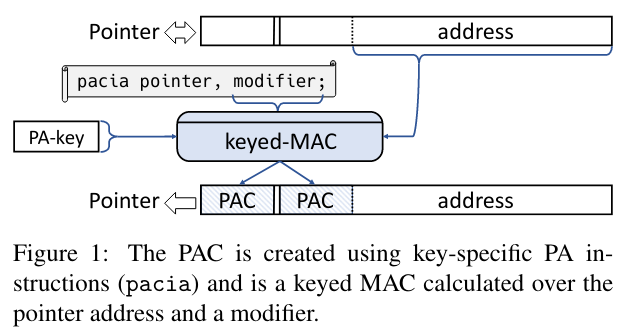
\includegraphics[width=\textwidth]{../cfi/arm-enc-ptr-fig}
\imagecredit{Liljestrand et al, ``PAC it up: Towards Pointer Integrity using ARM Pointer Authentication''}
\end{frame}

\begin{frame}{authentication keys}
    \begin{itemize}
    \item processes can have multiple authentication keys active
    \item easy to use separate keys for
        \begin{itemize}
        \item return address pointers
        \item function pointers
        \item any pointers to data
        \end{itemize}
    \item authentication keys are in special registers --- need OS to read/set
    \vspace{.5cm}
    \item also can ``mix'' in extra info like stack pointer
    \end{itemize}
\end{frame}

\begin{frame}{pointer authentication use}
    \begin{itemize}
    \item commonly enabled on ARM64 for return addreses
    \vspace{.25cm}
    \item otherwise:
    \item on ARM64 OS X --- used by OS X
        \begin{itemize}
        \item two different compiler `architectures': arm64, arm64e
        \item can't use arm64e libraries in arm64 program or vice-versa
        \end{itemize}
    \item proposals to use on Linux in global offset table, etc.
        \begin{itemize}
        \item GNU Linux linker option -z pac-plt; unclear if used `for real'
        \end{itemize}
    \end{itemize}
\end{frame}

\begin{frame}[fragile]{macOS PAC for apple code}
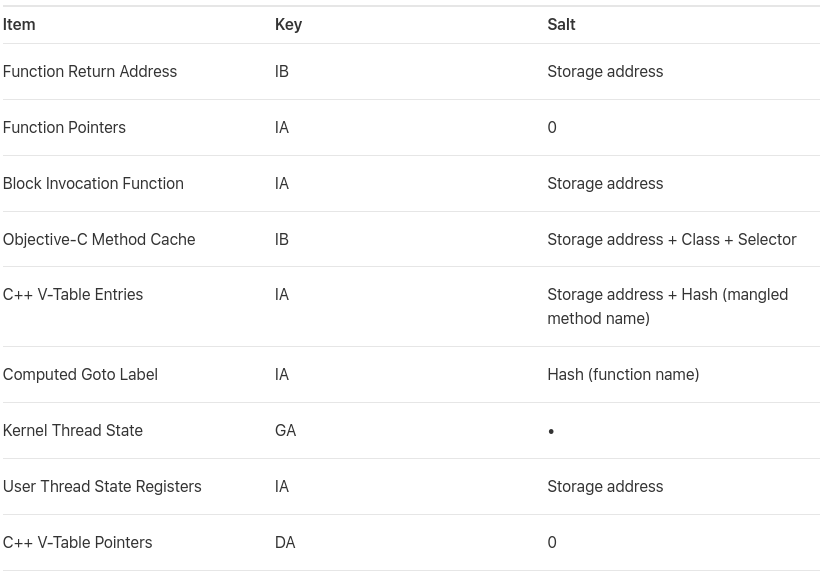
\includegraphics[height=0.9\textheight]{../cfi/apple-pac-usage}
\imagecredit{\url{https://support.apple.com/en-il/guide/security/sec8b776536b/1/web/1}}
\end{frame}

\begin{frame}{macOS PAC}
    \begin{itemize}
    \item `new' `preview' architecture in compiter
    \item seems to be used internally by Apple
    \item doesn't appear easily available/supported for others
    \item incompatible with `old' libraries
    \end{itemize}
\end{frame}

\begin{frame}{PAC bypasses}
    \begin{itemize}
    \item have been exploits in spite of PAC in iOS kernel
    \vspace{.5cm}
    \item only certain code pointers authenticated
        \begin{itemize}
        \item too expensive to authenticate all pointers
        \end{itemize}
    \item changing unsigned pointer values just before signed 
        \begin{itemize}
        \item get context switch to occur at just the right time
        \item modify pointer value in saved context
        \end{itemize}
    \item code that signs pointers they shouldn't
        \begin{itemize}
        \item changing pointer without crashing if old pointer invalid
        \end{itemize}
    \item `gadgets' that allow brute-forcing MAC tag
        \begin{itemize}
        \item not enough space in pointers for non-brute-forceable tag
        \end{itemize}
    \end{itemize}
\end{frame}

% FIXME
% FIXME: diagram

\end{document}
